\documentclass[crop=true]{standalone}
\usepackage{pgfplots}
\usepgfplotslibrary{fillbetween}
% \usetikzlibrary{angles}
\pgfplotsset{compat=1.15}

\begin{document}
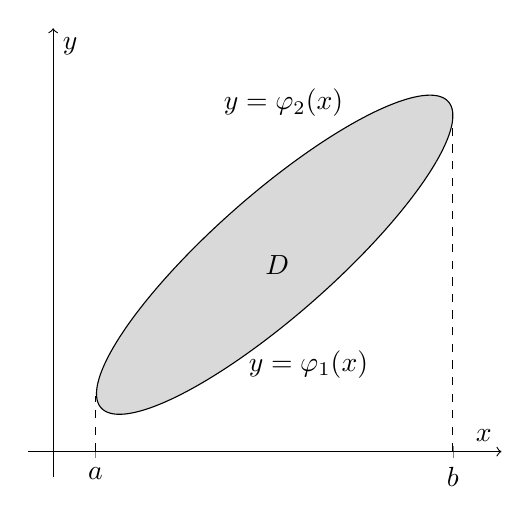
\begin{tikzpicture}[baseline]
\begin{axis}[
axis lines = middle,
unit vector ratio*=1 1 1,
scale=1.0, xmin=-0.2, xmax=3.6, ymin=-0.2, ymax=3.4,
%grid = major,
xtick={0.34,3.21},
ytick={0},
xticklabels = {$a$, $b$},
%yticklabels = {c,d},
xlabel=$x$,
ylabel=$y$,
axis line style = {->},
]
\addplot[name path=up,samples=100,domain=0:pi]({1.299*(cos(deg(x))+1) + 0.6*(sin(deg(x))+0.8)},{0.75*(cos(deg(x))+1) + 1.039*(sin(deg(x))+0.8)});
\addplot[name path=below,samples=100,domain=pi:2*pi]({1.299*(cos(deg(x))+1) + 0.6*(sin(deg(x))+0.8)},{0.75*(cos(deg(x))+1) + 1.039*(sin(deg(x))+0.8)});
\addplot[gray!30]fill between[of=up and below,soft clip={domain=-1:4}];
\draw[thin,dashed] (axis cs:0.34,0) -- (axis cs:0.34,0.45);
\draw[thin,dashed] (axis cs:3.21,0) -- (axis cs:3.21,2.75);
\node at (axis cs:1.8,1.5){$D$};
\node at (axis cs:2.05,0.7){$y=\varphi_1(x)$};
\node at (axis cs:1.85,2.8){$y=\varphi_2(x)$};
\end{axis}
\end{tikzpicture}

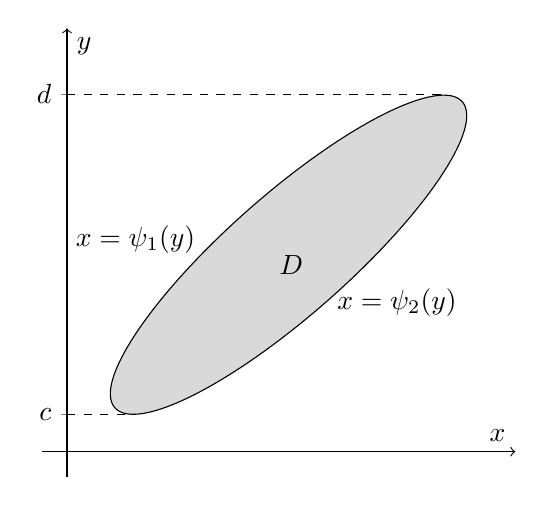
\begin{tikzpicture}[baseline]
\begin{axis}[
axis lines = middle,
unit vector ratio*=1 1 1,
scale=1.0, xmin=-0.2, xmax=3.6, ymin=-0.2, ymax=3.4,
%grid = major,
xtick={0},
ytick={0.3,2.87},
%xticklabels = {a,b},
yticklabels = {$c$, $d$},
xlabel=$x$,
ylabel=$y$,
axis line style = {->},
]
\addplot[name path=up,samples=100,domain=0:pi]({1.299*(cos(deg(x))+1) + 0.6*(sin(deg(x))+0.8)},{0.75*(cos(deg(x))+1) + 1.039*(sin(deg(x))+0.8)});
\addplot[name path=below,samples=100,domain=pi:2*pi]({1.299*(cos(deg(x))+1) + 0.6*(sin(deg(x))+0.8)},{0.75*(cos(deg(x))+1) + 1.039*(sin(deg(x))+0.8)});
\addplot[gray!30]fill between[of=up and below,soft clip={domain=-1:4}];
\draw[thin,dashed] (axis cs:0,0.3) -- (axis cs:0.48,0.3);
\draw[thin,dashed] (axis cs:0,2.87) -- (axis cs:3.05,2.87);
\node at (axis cs:1.8,1.5){$D$};
\node at (axis cs:0.55,1.7){$x=\psi_1(y)$};
\node at (axis cs:2.65,1.2){$x=\psi_2(y)$};
\end{axis}
\end{tikzpicture}

\end{document}